% Chapter 3

\chapter{Methodology} % Main chapter title

\label{Chapter3} % For referencing the chapter elsewhere, use \ref{Chapter1} 

%----------------------------------------------------------------------------------------

% Define some commands to keep the formatting separated from the content 
%\newcommand{\keyword}[1]{\textbf{#1}}
%\newcommand{\tabhead}[1]{\textbf{#1}}
%\newcommand{\code}[1]{\texttt{#1}}
%\newcommand{\file}[1]{\texttt{\bfseries#1}}
%\newcommand{\option}[1]{\texttt{\itshape#1}}

%----------------------------------------------------------------------------------------

The Design of the test bed can be broken down into several subsections. The lowest layer is made up of a USRP Software Defined Radio, connected to a computer over USB. On the computer, a Flask web server is started which connects this radio to a GNU Radio Flowgraph. The Flask server then connects the GNU Radio Flowgraph to the batman-adv mesh routing protocol. The Flask web server also configures a web interface that leverages SocketIO to allow for control and monitoring of the GNU Radio flowgraph. Finally, A.L.F.R.E.D. is configured by the web server as a means of sharing data among the nodes on the network. 

\begin{figure}
	\centering
	\includegraphics[scale=0.4]{ProtocolStack}
	\caption{An overview of the components of the system, including the OSI Layers they interact with.\cite{0003} \cite{0007} \cite{0008} \cite{0015} \cite{0012} \cite{0011}}
	\label{fig:ProtocolStack}
\end{figure}

This configuration is shown in Figure \ref{fig:ProtocolStack}

\section{SDR}

For ARCAM-Net, we utilized a combination of Ettus Research USRP B200 and USRP B210 SDRs. These radios are able to communicate from 70 MHz to 6 GHz and are well supported in GNU Radio using the open-source USRP Hardware Driver (UHD) provided by Ettus \cite{0007}. Their relatively low cost makes them ideal for building out larger testbeds. These serve as the radio transceiver for the current version of our platform. However, thanks to the UHD support in GNU Radio, any other USRP device will be compatible with the rest of the system, with little to no changes made to the development environment \cite{6737601}. 

\section{GNU Radio Flowgraph}

GNU Radio utilizes programs called ``Flowgraphs" to allow for graphical programming of SDR software. To implement the physical and link layers on the SDR, we utilize the Out of Tree (OOT) module gr-mac created by John Malsbury \cite{0015}. This flowgraph is an implementation of a Gaussian Minimum-Shift Keying (GMSK) and an Orthogonal Frequency-Division Multiplexing (OFDM) transceiver with a mac layer protocol called ``simple mac". There are two main blocks in the flowgraph. The first sets up the GMSK or OFDM radio. This hierarchical block is built by running a separate flowgraph which contains the UHD blocks to interface into the USRP as well as the modulation and demodulation blocks for the waveform. One of the more important aspects of the two radio blocks, is that they convert from streaming data to message data. 

Most features of GNU Radio work on streaming data where there is constant data transmission. However, packets are not sent continuously, therefore separate logic is needed to convert streams to messages. These messages are passed into and out of the GMSK and OFDM hierarchical blocks, so the remainder of the flowgraph deals with passing messages only \cite{6737601}. 

We use the GMSK block to convert from streaming data to message data and then connect this block to a tunnel (TUN) or network tap (TAP) interface block. TUN/TAP devices are virtual network kernel devices supported entirely in software. TUNs are used to simulate layer 3 devices and TAPs simulate layer 2 \cite{0017}. Either of these could be selected to suit the user's purpose, but as batman-adv is a layer 2 protocol, we will use the TAP protocol.

\section{Batman-adv}

Batman-adv was chosen based on its large community and documented success as a mesh routing protocol \cite{5375690}. It is already included as part of the Linux kernel, and additional software can be downloaded from most distributions repositories \cite{0008}. Configuring batman-adv to work on the SDR involves running the program batctl and selecting the recently generated TAP interface created by GNU Radio. The Maximum Transmission Unit (MTU) of the TAP interface must also be changed to 1532 from 1500 in order to incorporate the additional header batman-adv uses when sending data. Using only batman-adv and GNU Radio, we are able to create a Software Defined Radio based mesh network. The remainder of the test bed was implemented to leverage features unique to GNU Radio and batman-adv to create a method of sharing frequency and other data. 

\section{Flask Web Server and Socket.IO}

\begin{figure}
	\centering
	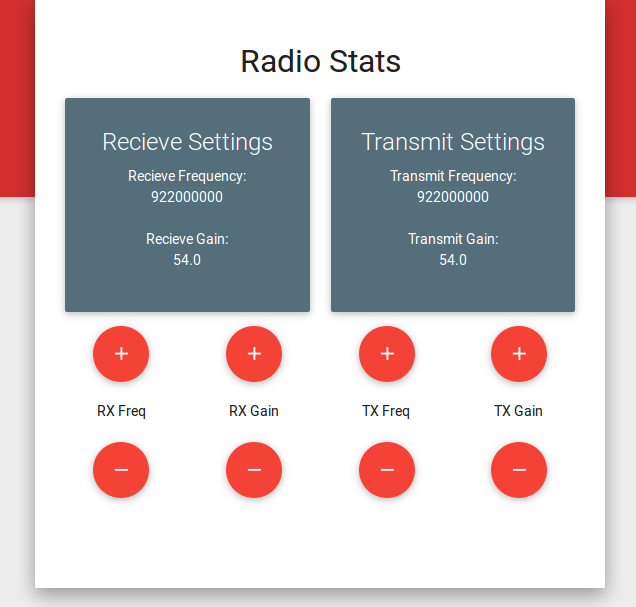
\includegraphics[scale=0.4]{WebInterFace}
	\caption{The web interface that lets the user initiate the network to hop to a new frequency.}
	\label{fig:WebInterface}
\end{figure}

Flask is a lightweight, open source, web framework for the Python programming language \cite{0011}. Flask was used to act as a broker between GNU Radio and any other user space applications or control systems we wished to implement. The Flask server runs the GNU Radio flowgraph in a background thread, while simultaneously configuring the TAP interface, setting up batman-adv, and starting A.L.F.R.E.D. as a background process. 

Socket.IO is a JavaScript library that enables real-time bidirectional event-based communication \cite{0012}.  SocketIO was chosen as a means of relaying data between the Flask server and other components of the system due to its speed, flexibility, and ability to broadcast messages to any connected client. Socket.IO also integrates into Flask \cite{0013} and can be used in stock Python with a client library \cite{0014}. In Flask, we create wrappers to all the necessary GNU Radio parameters so that external tools can relay data to and from GNU Radio over web sockets.  

We also use Flask to host a single webpage that displays various settings about the radio, and allows for the user to change parameters. The interface is shown in Figure \ref{fig:WebInterface}. Since our platform does not yet include logic for automatic detection of primary users, we simulate this by allowing a person to click a button to change to a new frequency. This frequency will then be sent to the Flask server using web sockets.  

\section{A.L.F.R.E.D.}

 The ``Almighty Lightweight Fact Remote Exchange Daemon," or A.L.F.R.E.D., is a system for distributing data to all nodes on a mesh network \cite{0015}. Whenever a node writes data to a channel on A.L.F.R.E.D., that data is passed between each node so that all members of the network receive the data. Typical uses for A.L.F.R.E.D. include keeping track of sensor data or building a visual map of the network. 

 An additional feature of A.L.F.R.E.D. is its ability to pass a command to the command line whenever new data is added \cite{0015}. When the transmission frequency of the USRP is changed on the Flask server, Flask sends this information along with a UTC timestamp to A.L.F.R.E.D. before changing frequencies. A small delay is created so that we can be sure the information was sent to the other nodes before the node changes its broadcast frequency.  

 When the other nodes receive the updated data table, A.L.F.R.E.D.'s callback function will run. This is a short program that parses the A.L.F.R.E.D. data table and looks for the most recent data it received. The callback function then sends the new frequency to Flask using Socket.IO which causes Flask to change the frequency in the GNU Radio flowgraph.   
%----------------------------------------------------------------------------------------

\section{Fabrication and Build Process}

The network was setup and run on a series of five Lenovo S30 Computers. All computers feature an Intel Xeon E5 processor and 32 GB of RAM. Each computer was running Ubuntu 14.04 LTS. The install process for GNU Radio, Batman-adv, and the rest of the technology stack is detailed in the appendix. Each computer was connected to one Ettus B200/B210 SDR using USB 3.0. 

All of the computers were connected together on a 10/100/1000 Ethernet router. This allowed for the control of the entire mesh to be handled by one computer. The popular terminal multiplexer Tmux was used in conjunction with SSH to send commands to all of the nodes in parallel. 

An additional Windows 10 laptop computer was used to control a Tektronix RSA306 wireless spectrum analyzer. This computer had an Intel i7 processor, and 8 GB of RAM. It is important to note that the RSA 306 requires a Windows machine, and therefore cannot be run on the same computer as the ones being used to run ARCAM-Net. This spectrum analyzer was used to confirm the operation of the radios and that frequency changes were occurring \cite{specan1}. 

%----------------------------------------------------------------------------------------

\section{Test Procedures}

\begin{figure}
	\centering
	\includegraphics[scale=0.4]{HopMessSmallest}
	\caption{The configuration used for the first set of tests.}
	\label{fig:HopMess}
\end{figure}

\begin{figure}
	\centering
	\includegraphics[scale=0.4]{NodeDrop}
	\caption{The configuration used for the second set of tests.}
	\label{fig:NodeDrop}
\end{figure}

In order to characterize the platform we ran three sets of tests presented below. The first test characterizes data hopping from one node to the next. The second test demonstrates batman-adv's ability to switch routes based on the quality of each node. The final tests were used to examine A.L.F.R.E.D.'s ability to be used for exchanging frequency information from node to node. 

\subsection{Network Benchmarks}
\label{network_benchmarks}

The first test was used to investigate the overhead each node adds to the network. To examine how adding hops affects the network, the USRPs were arranged so that each node was only able to directly connect to one or two neighboring nodes. This forced the nodes to need to use the multihop features of batman-adv in order to connect to the rest of the network. We used a total of 5 nodes as shown in Figure \ref{fig:HopMess}. We staggered the transmit and receive frequencies of the nodes to ensure that nodes could only talk to their immediate neighbors, forcing the network into the previously indicated configuration. The staggering of frequencies was needed to ensure each node would be unable to communicate to nodes other than its neighbors. 

 We then tested the setup at three different sets of frequencies, all within the Industrial, Scientific, and Medical (ISM) Band. We used different sets of ping tests in order to determine the number of dropped packets and the time it took to send the packets. We ran a standard ping test, one with reduced packet sizes, and one with increased time to live (TTL) settings. For a control group, two USRPs were connected together without batman-adv running. 


\subsection{Route Changes}

In a typical mesh environment, there will usually be more than one route from a source to a destination \cite{Akyildiz2009810}. In a traditional network, batman-adv switches routes based on the quality of each available link. The test was designed to determine if the same features would work in an SDRN. We initially set up four SDRs: a source, a destination, and two nodes to connect them. The first node is given a significantly larger gain in order to confirm that batman-adv will recognize that this is a more ideal path to the destination. Then, once the route is placed into the routing table, we lower the gain to 0 in order to force a transition to the other node. We then confirm that batman-adv is still able to find the new route. This setup is shown in Figure \ref{fig:NodeDrop}.



\subsection{Frequency Distribution}
\label{frequency_distribution}

In the final test, we tested to evaluate if A.L.F.R.E.D. would properly relay frequency changes over the mesh to other nodes. The user would increase or decrease the frequency using the web interface in order to simulate a cognitive radio making a decision to change to a new frequency. If A.L.F.R.E.D. was able to exchange the information properly, then the routing table would still show all connected nodes. We also used a Tektronix RSA306 Spectrum Analyzer in order to conclude that the transmission was occurring on the new frequency. If A.L.F.R.E.D. was not able to relay the information to all nodes, then some would change to the new frequency while others remain. This would be reflected in the output from the spectrum analyzer. 

%\subsection{Error (inaccuracy)}
%\subsection{Energy Use}

%----------------------------------------------------------------------------------------

%\section{Test - Network}

%\subsection{Signal Strength}
%\subsection{Range}
%\subsection{Noise}
%\subsection{Loss}
%\subsection{Error}
%\subsection{Energy Efficiency}
%\subsection{Latency}
%\subsection{Throughput}
%\subsection{Topology Effects}
%\subsection{Protocol}
%\subsection{Interference}
%\subsection{Crowding}
%\subsection{Crosstalk}

%----------------------------------------------------------------------------------------